%%%%%%%%%%%%%%%%%%%%%%%%%%%%%%%%%%%%%%%%%
% Short Sectioned Assignment LaTeX Template Version 1.0 (5/5/12)
% This template has been downloaded from: http://www.LaTeXTemplates.com
% Original author:  Frits Wenneker (http://www.howtotex.com)
% License: CC BY-NC-SA 3.0 (http://creativecommons.org/licenses/by-nc-sa/3.0/)
%%%%%%%%%%%%%%%%%%%%%%%%%%%%%%%%%%%%%%%%%

%----------------------------------------------------------------------------------------
%	PACKAGES AND OTHER DOCUMENT CONFIGURATIONS
%----------------------------------------------------------------------------------------

\documentclass[paper=a4, fontsize=11pt]{scrartcl} % A4 paper and 11pt font size

% ---- Entrada y salida de texto -----

\usepackage[T1]{fontenc} % Use 8-bit encoding that has 256 glyphs
\usepackage[utf8]{inputenc}
%\usepackage{fourier} % Use the Adobe Utopia font for the document - comment this line to return to the LaTeX default

% ---- Idioma --------

\usepackage[spanish, es-tabla]{babel} % Selecciona el español para palabras introducidas automáticamente, p.ej. "septiembre" en la fecha y especifica que se use la palabra Tabla en vez de Cuadro

% ---- Otros paquetes ----

\usepackage{url} % ,href} %para incluir URLs e hipervínculos dentro del texto (aunque hay que instalar href)
\usepackage{hyperref}
\hypersetup{
	colorlinks=true,
	linkcolor=black,
	urlcolor=black,
	citecolor=black,
}
\usepackage{amsmath,amsfonts,amsthm} % Math packages
%\usepackage{graphics,graphicx, floatrow} %para incluir imágenes y notas en las imágenes
\usepackage{graphics,graphicx, float} %para incluir imágenes y colocarlas

% Para hacer tablas comlejas
%\usepackage{multirow}
%\usepackage{threeparttable}

%\usepackage{sectsty} % Allows customizing section commands
%\allsectionsfont{\centering \normalfont\scshape} % Make all sections centered, the default font and small caps

\usepackage{fancyhdr} % Custom headers and footers
\pagestyle{fancyplain} % Makes all pages in the document conform to the custom headers and footers
\fancyhead{} % No page header - if you want one, create it in the same way as the footers below
\fancyfoot[L]{} % Empty left footer
\fancyfoot[C]{} % Empty center footer
\fancyfoot[R]{\thepage} % Page numbering for right footer
\renewcommand{\headrulewidth}{0pt} % Remove header underlines
\renewcommand{\footrulewidth}{0pt} % Remove footer underlines
\setlength{\headheight}{13.6pt} % Customize the height of the header

\numberwithin{equation}{section} % Number equations within sections (i.e. 1.1, 1.2, 2.1, 2.2 instead of 1, 2, 3, 4)
\numberwithin{figure}{section} % Number figures within sections (i.e. 1.1, 1.2, 2.1, 2.2 instead of 1, 2, 3, 4)
\numberwithin{table}{section} % Number tables within sections (i.e. 1.1, 1.2, 2.1, 2.2 instead of 1, 2, 3, 4)

\setlength\parindent{0pt} % Removes all indentation from paragraphs - comment this line for an assignment with lots of text

\newcommand{\horrule}[1]{\rule{\linewidth}{#1}} % Create horizontal rule command with 1 argument of height
\usepackage{booktabs}

\usepackage{listings}
\lstdefinelanguage
[x64]{Assembler}     % add a "x64" dialect of Assembler
[x86masm]{Assembler} % based on the "x86masm" dialect
{morekeywords={CDQE,CQO,CMPSQ,CMPXCHG16B,JRCXZ,LODSQ,MOVSXD, %
		POPFQ,PUSHFQ,SCASQ,STOSQ,IRETQ,RDTSCP,SWAPGS, %
		rax,rdx,rcx,rbx,rsi,rdi,rsp,rbp, %
		r8,r8d,r8w,r8b,r9,r9d,r9w,r9b, %
		r10,r10d,r10w,r10b,r11,r11d,r11w,r11b, %
		r12,r12d,r12w,r12b,r13,r13d,r13w,r13b, %
		r14,r14d,r14w,r14b,r15,r15d,r15w,r15b}} % etc.
\usepackage{color}
\usepackage{xcolor}
\lstdefinestyle{customc}{
	belowcaptionskip=1\baselineskip,
	breaklines=true,
	frame=L,
	xleftmargin=\parindent,
	language=C,
	showstringspaces=false,
	basicstyle=\footnotesize\ttfamily,
	keywordstyle=\bfseries\color{green!40!black},
	commentstyle=\itshape\color{purple!40!black},
	identifierstyle=\color{blue},
	stringstyle=\color{orange},
}

\lstset{escapechar=@,style=customc}
\usepackage{url}


\title{	
	\normalfont \normalsize
	\begin{figure}[htb]
		\centering
		
\includegraphics[width=0.3\textwidth]{./imagenes/1}
	\end{figure}
	\textsc{\textbf{Estructura de Computadores} \\ Grado en Ingeniería Informática \\ 
	Curso 2018-2019} \\ [25pt] % Your university, school and/or department name(s)
	\begin{figure}[htb]
		\centering
		
\includegraphics[width=0.15\textwidth]{./imagenes/2}
	\end{figure}
	\horrule{0.5pt} \\[0.4cm] % Thin top horizontal rule
	\huge Memoria Práctica 6. \\
	\huge Caché.
	\\ % The assignment title
	\horrule{2pt} \\[0.5cm] % Thick bottom horizontal rule
}
\author{Félix Ramírez García  \\
\href{mailto:felixramirezgarcia@correo.ugr.es}{felixramirezgarcia@correo.ugr.es}} % Nombre y apellidos
\date{\normalsize\today} % Incluye la fecha actual

%----------------------------------------------------------------------------------------
% DOCUMENTO
%----------------------------------------------------------------------------------------

\begin{document}
	
	\maketitle % Muestra el Título
	
	\newpage %inserta un salto de página
	
	\tableofcontents % para generar el índice de contenidos
	
	\listoffigures % para generar índice de imágenes.
	
	\listoftables % para generar índice de tablas.
	
	\newpage
	
	%-----------------------------------------------------------------------
	%				   	Códigos de los programas
	%-----------------------------------------------------------------------
	\section[Códigos de los programas]{Códigos de los programas}
	
	\subsection{Programa line.cc}
	
	\lstset{language=C}
	\begin{lstlisting}[frame=single]
#include <algorithm>    // nth_element
#include <array>        // array
#include <chrono>       // high_resolution_clock
#include <iomanip>      // setw
#include <iostream>     // cout
#include <vector>       // vector

using namespace std::chrono;

const unsigned MAXLINE = 1024; // maximun line size to test
const unsigned GAP = 12;       // gap for cout columns
const unsigned REP = 100;      // number of repetitions of every test

int main(){
	std::cout << "#" 
	<< std::setw(GAP - 1) << "line (B)"
	<< std::setw(GAP    ) << "time (nanosegundos)"
	<< std::endl;

	for (unsigned line = 1; line <= MAXLINE; line <<= 1){
		std::vector<duration<double, std::micro>> score(REP);
	
		for (auto &s: score){
			std::vector<char> bytes(1 << 24); // 16MB
	
			auto start = high_resolution_clock::now();
	
			for (unsigned i = 0; i < bytes.size(); i += line)
				bytes[i] ^= 1;
	
			auto stop = high_resolution_clock::now();
	
			s = stop - start;
		}

		std::nth_element(score.begin(), 
		score.begin() + score.size() / 2, 
		score.end());

		std::cout << std::setw(GAP) << line
		<< std::setw(GAP) << std::fixed << std::setprecision(1)
		<< std::setw(GAP) << score[score.size() / 2].count()
		<< std::endl;
	}
}
	\end{lstlisting}
	
	\subsection{Programa size.cc}
	
	\lstset{language=C}
	\begin{lstlisting}[frame=single]
#include <algorithm>    // nth_element
#include <array>        // array
#include <chrono>       // high_resolution_clock
#include <iomanip>      // setw
#include <iostream>     // cout
#include <vector>       // vector

using namespace std::chrono;

const unsigned MINSIZE = 1 << 10; // minimun line size to test:  1KB
const unsigned MAXSIZE = 1 << 26; // maximun line size to test: 32MB
const unsigned GAP = 12;          // gap for cout columns
const unsigned REP = 100;         // number of repetitions of every test
const unsigned STEPS = 1e6;       // steps

int main() {
	std::cout << "#" 
	<< std::setw(GAP - 1) << "line (B)"
	<< std::setw(GAP    ) << "time (nanosegundos)"
	<< std::endl;
	
	for (unsigned size = MINSIZE; size <= MAXSIZE; size *= 2){
		std::vector<duration<double, std::micro>> score(REP);
		
		for (auto &s: score){
			std::vector<char> bytes(size);
			unsigned tamanio = size -1;
			auto start = high_resolution_clock::now();
			
			for (unsigned i = 0; i < STEPS; ++i)
				bytes[(i*64)&(size-1)] ^= 1;
			
			auto stop = high_resolution_clock::now();
			
			s = stop - start;
		}
		
		std::nth_element(score.begin(), 
		score.begin() + score.size() / 2, 
		score.end());
		
		std::cout << std::setw(GAP) << size
		<< std::setw(GAP) << std::fixed << std::setprecision(1)
		<< std::setw(GAP) << score[score.size() / 2].count()
		<< std::endl;
	}
}
	\end{lstlisting}
	
	%-----------------------------------------------------------------------
	%				   			Gráficas
	%-----------------------------------------------------------------------
	\section[Gráficas]{Gráficas}
	
	A continuación se muestran las gráficas generadas con los programas anteriores. \\
	
	La figura 2.1 muestra que cuanto mas grande es el tamaño, menos tiempo tarda en ejecutarse. Tiene un punto de inflexión en 16 B, donde cambia el sentido de la función.
	
	\begin{figure}[htb]
		\centering
		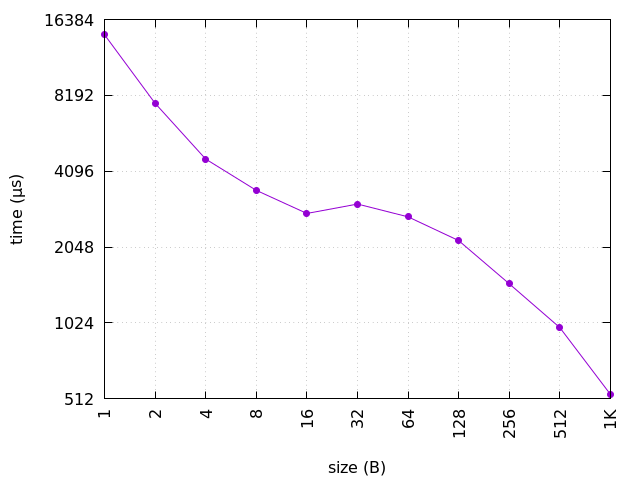
\includegraphics[width=1.0\textwidth]{./imagenes/line}
		\caption{Grafica obtenida por la ejecucion de line.cc.} \label{fig:1}
	\end{figure}
	
	En la figura 2.2 se puede apreciar que se mantiene un tiempo constante hasta llegar a un tamaño de 32K, y a partir de hay va incrementando gradualmente hasta 8 M donde parece que se vuelve a mantener constante. Cabe destacar que entre 64K y 256K no hay un incremento significativo. El mayor incremento de tiempo se produce entre 2 y 4 M.
	
	\begin{figure}[htb]
		\centering
		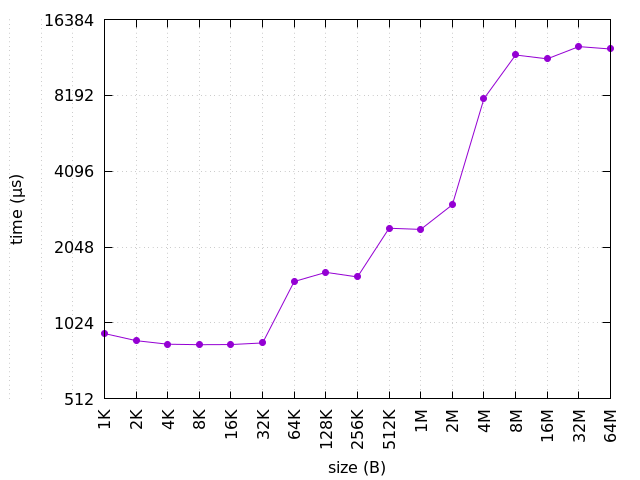
\includegraphics[width=1.0\textwidth]{./imagenes/size}
		\caption{Grafica obtenida por la ejecucion de size.cc.} \label{fig:1}
	\end{figure}
	
	%-----------------------------------------------------------------------
	%				   	Caracteristicas de nuestra CPU
	%-----------------------------------------------------------------------
	\section[Caracteristicas de nuestra CPU]{Caracteristicas de nuestra CPU}
	
	Las características de nuestra CPU son las obtenidas con el comando lscpu. Son las siguientes:
	
	\lstset{language=C}
	\begin{lstlisting}[frame=single]
Arquitectura:                        x86_64
modo(s) de operacion de las CPUs:    32-bit, 64-bit
Orden de los bytes:                  Little Endian
CPU(s):                              1
Lista de la(s) CPU(s) en linea:      0
Hilo(s) de procesamiento por nucleo: 1
Nucleo(s) por socket:                1
Socket(s)                            1
Modo(s) NUMA:                        1
ID de fabricante:                    GenuineIntel
Familia de CPU:                      6
Modelo:                              142
Nombre del modelo:                   Intel(R) Core(TM) i3-7100U CPU 2.40GHz
Revision:                            9
CPU MHz:                             2399.998
BogoMIPS:                            4799.99
Fabricante del hipervisor:           KVM
Tipo de virtualizacion:              lleno
Cache L1d:                           32K
Cache L1i:                           32K
Cache L2:                            256K
Cache L3:                            3072K
CPU(s) del nodo NUMA 0:              0
Indicadores:                         fpu vme de pse tsc msr pae mce cx8 
				 apic sep mtrr pge mca cmov pat pse36 
				 clflush mmx fxsr sse sse2 syscall nx 
				 rdtscp lm constant_tsc rep_good nopl 
				 xtopology nonstop_tsc cpuid pni 
				 pclmulqdq monitor ssse3 cx16 pcid 
				 sse4_1 sse4_2 x2apic movbe popcnt aes
				 xsave avx rdrand hypervisor lahf_lm 
				 3dnowprefetch invpcid_single pti fsgsbase
				 avx2 invpcid rdseed clflushopt abm
	\end{lstlisting}
		
	%-----------------------------------------------------------------------
	%							BIBLIOGRAFIA
	%-----------------------------------------------------------------------
	% Referencia a bibliografia			En \cite{Baz}
	% Referencia a figura				La figura (\ref{fig:1})
	% Espacio entre lineas				\vspace{0.06in}
	% Figura con comentario al pie
	%\begin{figure}[htb]
	%	\centering
	%	
\includegraphics[width=0.4\textwidth]{./imagenes/1}
	%	\caption{Universidad de Granada.} \label{fig:1}
	%\end{figure}
	%\begin{thebibliography}{99}
	%	\bibitem{Baz} 
	%	\textsc{Bazaraa, M.S., J.J. Jarvis}
	%	\textit{Programacuib}.
	%	\newline
	%	\url{https://www.google.es}	
	%\end{thebibliography}

	


\end{document}